\chapter{Revisão de Literatura}
\label{sec:revisao}

\section{Redes Sociais e Análise de Redes Sociais: desvendando vínculos e transferências}

Uma rede social é uma estrutura composta por indivíduos ou organizações. Cada um deles é denominado nó e podem ser conectados por um ou mais tipos de interdependência, como amizade, interesses comuns, troca financeira, relacionamento sexual, conhecimento ou prestígio social \cite{kadushin2005benefits}.

A análise de rede social enxerga o relacionamento social considerando a teoria dos grafos, onde os principais elementos são os nós e ligações (também conhecidas por enlaces ou conexões). Os nós são os atores dentro de uma rede social e as ligações representam os relacionamentos entre eles \cite{kadushin2005benefits}.

Muitas vezes, a rede social pode apresentar uma estrutura complexa pois podem existir diversos tipos diferentes de relacionamentos. As rede sociais podem funcionar em diversos níveis de complexidade e podem ser determinantes na forma como os problemas comuns são resolvidos. \cite{stanley1994social}.

\section{Rede Social}
O entendimento dos relacionamentos entre atores é fundamental para a compreensão de fenômenos sociais. Como uma doença se espalha ou como as pessoas podem ser influenciadas são exemplos de situações onde a compreensão das interações sociais são relevantes. Nesta seção serão apresentadas as principais definições no campo das redes sociais.

Uma rede social é definida como uma representação visual do relacionamento entre pessoas ou organizações. Cada nó (ator ou vértice) representa um indivíduo ou grupo de indivíduos. Um enlace (relacionamento) conecta dois nós, o quê representa visualmente o relacionamento entre eles.

O uso de grafos para representar essa estrutura social possibilitar uma análise rigorosa da informações intrínsecas na rede. Os conceitos da teoria dos grafos garantem o uso rigoroso de metodologias de análise para identificar e medir as correlações entre as entidades \cite{pan2007effective}.

Para facilitar o entendimento de uma rede social considere o seguinte exemplo: Os profissionais de uma unidade hospitalar necessitam abrir vaga de internação na unidade renal para uma paciente crítico. Para isso, eles precisam identificar um paciente estável da unidade renal que possa ser transferido. Neste caso, a equipe precisa trabalhar em conjunto, trocando informações em sua rede social para resolver dois problemas: (1) Identificar qual paciente pode ser transferido e (2) Identificar uma unidade que pode receber o paciente estável.

Partindo desta situação, foram coletadas informações sobre a interação dos atores para conseguir resolver o problema de abertura de vaga para o paciente crítico. A tabela \ref{table:social-network-example} sumariza os dados coletados sobre a rede social hipotética considerada. 

Os atores identificados foram: 1) Enf. Em. (Enfermeira da Emergência), (2) Méd. Em. (Médico da Emergência), (3) Enf. Renal (Enfermeira da Unidade Renal), (4) Méd. Renal (Médico da Unidade Renal), (5) Enf. Neo (Enfermeira da Unidade Neonatal) e (6) Méd. Neo (Médico da Unidade Neonatal). O relacionamento entre os atores é representado da seguinte forma: 1 quando existir ou 0 quando não existir.

\begin{table}[htbp]
\centering
\caption{Exemplo de rede social em uma unidade hospitalar}
\label{table:social-network-example}
\begin{tabular}{|l|l|l|l|l|l|l|}
\hline
                                      & Enf. Em. & Enf. Renal & Méd. Em. & Méd. Renal & Enf. Neo & Méd. Neo \\ \hline
Enf. Em.                 & 0                     & 1                                   & 1                 & 0                       & 0                                     & 0                                 \\ \hline
Enf. Renal   & 0                     & 0                                   & 0                 & 1                       & 1                                     & 0                                 \\ \hline
Méd. Em.                     & 1                     & 1                                   & 0                 & 1                       & 0                                     & 0                                 \\ \hline
Méd. Renal               & 1                     & 0                                   & 1                 & 0                       & 1                                     & 1                                 \\ \hline
Enf. Neo & 0                     & 1                                   & 0                 & 0                       & 0                                     & 1                                 \\ \hline
Méd. Neo     & 0                     & 0                                   & 0                 & 1                       & 1                                     & 0                                 \\ \hline
\end{tabular}
\end{table}

Na Figura \ref{fig:social-network-example}, cada nó representa um profissional do hospital e a ligação representa o relacionamento entre eles na resolução do problema. A direção da comunicação dos nós é do início para o fim da seta.

\begin{figure}[htbp]
\centering
 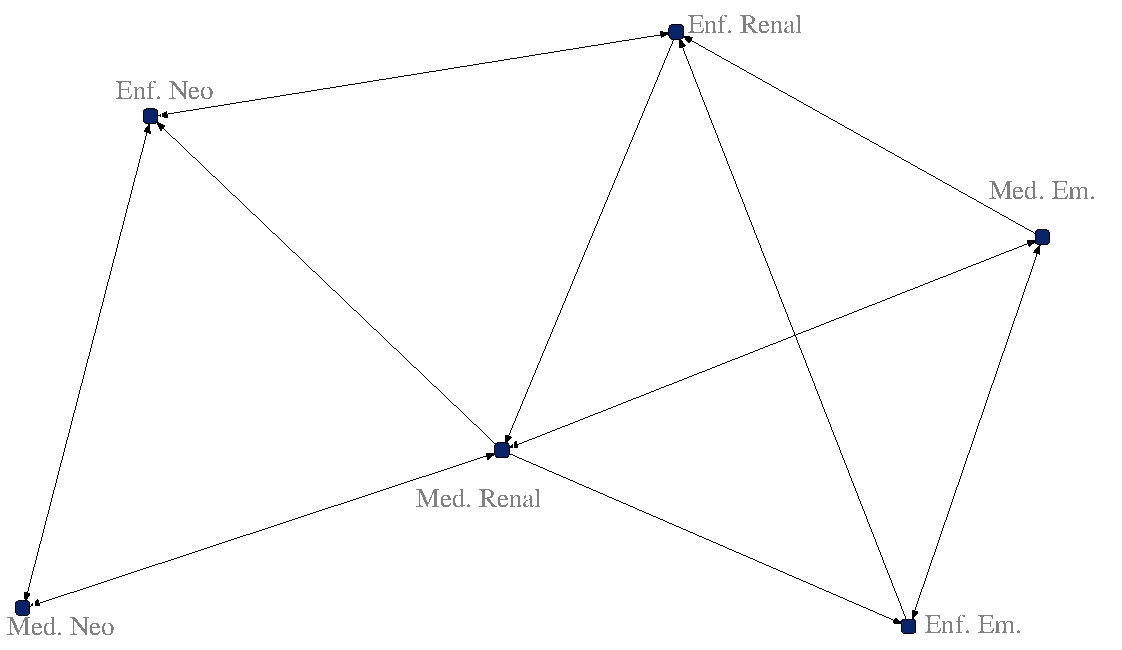
\includegraphics[width=\textwidth]{figuras/rede-exemplo.pdf}
 \caption{Representação visual da rede social hipotética}
\label{fig:social-network-example}
\end{figure}

\subsection{Obtenção de Dados}
Segundo \cite{de2011exploratory}, as informações de relacionamento de uma rede social podem ser coletadas utilizando duas técnicas principais: (1) Elicitação e (2) Registro. A primeira usa questionários como fonte de informações, enquanto que a segunda extrai os dados através de lista de membros, registro de emails, artigos científicos etc.

Os questionários, no início das pesquisas em redes sociais, eram o método principal para obtenção de informações. Neste método, pede-se aos atores que respondam questões sobre as interações que eles realizam na solução de problemas. Porém, segundo \cite{pastor2003statistical,carrington2005models,newman2003ego}, este tipo de técnica pode levar a obtenção de informações imprecisas. Além disso, este método requer muito esforço para ser alcançado o que pode acabar limitando o tamanho da rede estudada. 

O segundo método utiliza dos recursos de computação (redes de computadores, compartilhamento de informações, internet) para obtenção de informações de forma automática. Por exemplo, quando pesquisadores publicam um artigo há uma relação de colaboração entre eles, que pode ser usada na criação da rede social focada em pesquisa científica. Entretanto, em alguns casos, a interpretação destes dados necessita de mais atenção para entender melhor como o relacionamento dos atores está ocorrendo.

\subsection{Tipos de Redes Sociais}
As redes sociais podem ser classificadas levando em conta seus atributos no que diz respeito aos nós e ligações. Os nós, por exemplo, podem possuir pesos, que indicam sua importância na rede. Assim como os nós, as ligações também podem possuir pesos diferentes \cite{pan2007effective}. 

Por exemplo, em uma rede social hospitalar, os atores podem indicar o grau de importância nas relações com outros atores através de um valor entre 0 a 5. Além disso, as ligações podem ser não-simétricas, ou seja, um ator A pode indicar um ator B, mas o último não indicar o primeiro como integrante de suas relações (ligações direcionadas). Ligações simétricas existem quanto há uma relacionamento em ambas as direções, ou seja, de A para B e de B para A.

A figura \ref{fig:graph-types} exibe alguns exemplos diferentes de redes sociais.

\begin{figure}[htbp]
\centering
 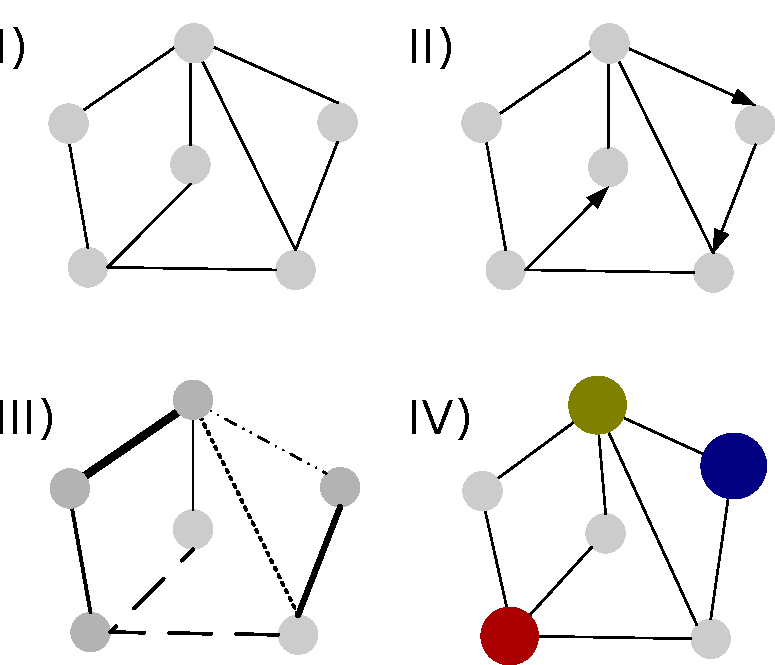
\includegraphics[width=.85\textwidth]{figuras/tipos.pdf}
 \caption{Exemplo de diferentes redes sociais. I) Possui apenas um tipo de nó e de ligações não direcionadas. II) Rede com ligações direcionadas e não direcionadas. III) Rede com ligações com pesos distintos e IV) Rede com nós de tipos e pesos diferentes.}
\label{fig:graph-types}
\end{figure}

\subsection{Análise de Rede Social: Caminhos em Produção}
A análise de rede social surgiu como uma técnica moderna da sociologia e acabou ganhando reconhecimento na antropologia, biologia, economia, saúde etc. Ela pode ser definida como, segundo \cite{krebs2015}, ``O Mapeamento e medição do relacionamento e fluxos entre pessoas, grupos, organizações, computadores e outras informações das entidades.''

O Estudo das redes sociais se interessa primordialmente pelas interações entre os atores, ou seja, as análises são feitas em cima das ligações. Porém, isto não invalida a importância das características dos atores \cite{pan2007effective}.

As análises verificam as propriedades estruturais dos indivíduos ou grupos de indivíduos na rede, por exemplo: como os atores estão conectados aos outros, como os atores afetam as conexões dos outros ou mesmo como os grupos de atores estão conectados à rede.

\subsubsection{Algumas Métricas Utilizadas na Análise de Redes Sociais}
Nesta subseção serão listadas algumas métricas que podem ser utilizadas na análise de redes sociais.

\begin{itemize}
 \item Grau de Intermediação (Betweenness): Esta métrica leva em conta a conectividade dos nós da rede. Quanto maior o grau de intermediação de um nó, maior o nível de propragação de informações na rede.
 \item Ponte (Bridge): Uma ligação é dita do tipo ponte quando a sua remoção resulta na separação da rede em grupos diferentes.
 \item Centralidade (Centrality): Indica a importância social de um nó na conexão da rede.
 \item Grau de Proximidade (Closeness): Reflete o grau de proximidade de um ator da rede aos outros, ou seja, indica a habilidade dele acessar informações de outros atores direta ou indiretamente.
 \item Coeficiente de Agrupamento (Clustering Coefficient): Indica a probabilidade de dois atores ligados a um terceiro poderem se associar.
 \item Coesão (Cohesion): No contexto de grupos sociais, um grupo está coeso quando seus membros possuem laços ligando-os uns aos outros e ao grupo como um todo. Os membros de grupos fortemente coesos estão mais inclinados a permanecer nele.
 \item Grau (Degree): Indica o número de vínculos com outros atores na rede.
 \item Centralidade de Intermediação de Fluxo (Flow betweenness centrality): Medida que um nó contribui para à soma do fluxo máximo entre todos os pares de nós.
 \item Centralidade Eigenvector (Eigenvector centrality): É a medida de importância de um nó na rede.
\end{itemize}

\subsection{Redes Sociais e a Saúde: Entrelaçamentos para o Cuidar}
A análise de redes sociais na saúde constitui um campo de grande interesse. Através das redes de relacionamento, por exemplo, comunidades podem buscar melhorias na sua realidade, inclusive na melhoria do acesso à saúde. Tais iniciativas buscam promover apoio social, compartilhar experiências e oferecer serviços de cuidados à saúde. Estas ações podem facilitar a resolução de problemas, dando poder às comunidades para que elas possam lidar com os problemas locais \cite{maior2004formaccao}. Observa-se um forte componente de contribuição para o empoderamento de sujeitos e autonomização para tomada de decisão. 

As redes sociais desenvolvem ações solidárias para lidar com questões do cotidiano entre grupos menos favorecidos, e fortalecem o sentimento de participação de um grupo social. \cite{de2002apoio}. São estruturantes nos movimentos de produção de sentidos para produção da saúde, da educação e de tantos outros elementos necessários ao sujeito.

A saúde pode ser entendida como um produto de interações humanas, e a partir daí, ela pode ser definida a partir de determinantes sociais, afetivos, culturais, econômicos etc. \cite{martins2004redes}.

Além do importante papel que a rede social apresenta no cunho social, sua importância também se revela nas interações dos profissionais da saúde.  A troca de experiências, o comprometimento da equipe na resolução de problemas comuns, podem contribuir no atendimento da população, pois garantem o acesso aos serviços de saúde e respostas as demandas dos usuários de forma integral e interdisciplinar.

\section{O cuidado a Hipertensos e Diabéticos na Atenção Básica}
A \acrlong{HAS} é uma condição clínica multifatorial caracterizada por níveis elevados e sustentados de \acrlong{PA} – PA (PA $\geq$ 140 x 90 mmHg). Está associada às mudanças na função e/ou na estrutura de órgãos-alvo e também a mudanças no metabolismo, levando a um aumento no risco de problemas cardiovasculares. \cite{hipertenso}.

A HAS é um problema de saúde pública preocupante no Brasil, pois tem prevalência alta entre 22\% e 44\% para adultos (32\% em média), alcançando mais de 50\% da população de indivíduos com 60 a 69 anos e 75\% em indivíduos com mais de 70 anos \cite{hipertenso}.

No Brasil, as equipes da AB estão geralmente ligadas às ações de controle e prevenção da HAS e de suas complicações. As equipes multiprofissionais devem desenvolver seu processo de trabalho estabelecendo vínculo com a comunidade e considerando diversidade racial, cultural, religiosa e os demais fatores sociais e/ou determinantes envolvidos a cada indivíduo. Para o Ministério da Saúde, fatores relacionados ao estilo de vida são essenciais para melhor desenvolvimento da terapia e prevenção da hipertensão. \cite{atencaobasica37}.

Para a Sociedade Brasileira de Cardiologia (2010) os hábitos saudáveis de vida devem ser adotados ainda na infância e adolescência, tendo como principais medidas não-farmacológicas para a prevenção da HAS a alimentação saudável, o consumo controlado de sódio e álcool, a ingestão de potássio e o combate ao sedentarismo e ao tabagismo. E os fatores de risco são a idade, gênero e etnia, excesso de peso e obesidade, ingestão de sal, ingestão de álcool, sedentarismo, fatores socioeconômicos, genética e outros comprometimentos vasculares. \cite{hipertenso}.

\cite{da2012associaccao}, colocam a HAS como uma doença crônica, também conhecida como ``assassina silenciosa'', já que na maioria das vezes, ela não apresenta sintomas, o que dificulta seu diagnóstico e a adesão ao tratamento. Essa adesão envolve ações de hábitos saudáveis, o que muitas vezes sucinta a mudança de estilos de vida. Tarefa nem sempre fácil ou bem aceita pelos pacientes e suas famílias. 

Pela PNAB \cite{ministerio2012politica}, as atribuições do Enfermeiro na AB são: realizar consulta de enfermagem, procedimentos, atividades em grupo e conforme protocolos ou outras normativas técnicas estabelecidas pelo gestor federal, estadual, municipal ou do Distrito Federal, observadas as disposições legais da profissão, solicitar exames complementares, prescrever medicações e encaminhar, quando necessário, usuários a outros serviços. 

Destacando a consulta de enfermagem, esta é importante para o acompanhamento da pessoa com diagnóstico de HAS e deve ser realizada com aplicação da \acrlong{SAE} (\acrshort{SAE}) \cite{atencaobasica37}, que segundo a Resolução do Cofen, nº 358, de 15 de outubro 2009, é composta pelo histórico, exame físico, diagnóstico das necessidades de cuidado da pessoa, planejamento da assistência (incluindo a prescrição de cuidados e um plano terapêutico construído com a pessoa); implementação da assistência e avaliação do processo de cuidado (inclui a avaliação contínua e conjunta com a pessoa e com a família em relação aos resultados do tratamento e do desenvolvimento ao longo do processo de apoio ao autocuidado).e possui seis etapas interrelacionadas entre si, objetivando a educação em Saúde para o autocuidado. \cite{de2009resoluccao}.

Esta consulta deve se focar nos fatores de risco que influenciam o controle da hipertensão, ou seja, as mudanças no estilo de vida, o incentivo à atividade física, à redução do peso corporal quando acima do \acrlong{IMC} (\acrshort{IMC}) recomendado e o abandono do tabagismo. Deve também estar voltada para as possibilidades de fazer a prevenção secundária, a manutenção de níveis pressóricos abaixo da meta e o controle de fatores de risco.

O sucesso dessas ações vai depender em suma, do vínculo entre profissional e paciente, estabelecendo pactuações e corresponsabilização. Para garantir isso, o profissional deve ter em mente que o momento da consulta é também um momento de educação em saúde, um momento de partilha de saberes.

\cite{santos2012adesao}, coloca que para haver o desenvolvimento do conhecimento sobre saúde-doença faz-se necessário haver profissionais voltados à educação, mas que sejam aliados dos pacientes na tarefa de encorajá-los a respeito do autocuidado e de desenvolverem o senso de responsabilidade de proteção a própria saúde. 

As ações de educação em saúde também devem contar com a participação dos demais membros da equipe de saúde, criando assim, uma maior atmosfera de apoio e comprometimento de todos. 

As necessidades que estes pacientes demandam, envolvem o trabalho do enfermeiro tanto no desempenho de suas ações assistenciais quanto gerenciais. Os aspectos gerenciais envolvem a comunidação efetiva com a equipe e também outros profissionais e serviços externos a unidade. Assim, profissionais bem articulados em suas relações, favorecem um acompanhamento mais satisfatório desses pacientes. 

Com relação ao \acrlong{DM}, esta patologia encontra-se por vezes associada ao quadro de HAS, uma vez que o DM pode levar a alterações vasculares, colaborando para o desenvolvimento de HAS. A hipertensão arterial sistêmica afeta a maioria dos portadores de diabetes. É fator de risco importante para a doença coronariana e para as complicações microvasculares como a retinopatia e a nefropatia. \cite{atencaobasica16}.

O termo ``Diabetes Mellitus'' trata-se de um transtorno metabólico de etiologias heterogêneas, caracterizado por hiperglicemia e distúrbios no metabolismo de carboidratos, proteínas e gorduras, resultantes de defeitos da secreção e/ou da ação da insulina \cite{assal1999definition}.

Os efeitos do diabetes mellitus incluem danos de longo prazo, disfunção e falha de vários órgãos. DM pode estar presente com sintomas característicos como sede, poliúria, visão embaçada e perda de peso. \cite{assal1999definition}.

Frequentemente os sintomas podem não ser severos ou mesmo podem estar ausentes e consequentemente, a hiperglicemia  necessária para causar alterações patológicas e funcionais pode estar presente por um longo tempo antes de diagnosticada. \cite{assal1999definition}.

De acordo com a Sociedade Brasileira de Diabetes (2014), uma epidemia de diabetes mellitus está em curso. Em 1985, estimava-se haver 30 milhões de adultos com DM no mundo; esse número cresceu para 135 milhões em 1995, atingindo 173 milhões em 2002, com projeção de chegar a 300 milhões em 2030. \cite{sarah2004global}.

No Brasil, dados da Vigilância de Fatores de Risco e Proteção para Doenças Crônicas por Inquérito Telefônico (Vigitel), de 2011, mostram que a prevalência de diabetes referida pela própria  população acima de 18 anos aumentou de 5,3\% para 5,6\%, entre 2006 e 2011. Quanto ao gênero, a análise mostrou um aumento de casos entre os homens, que eram 4,4\%, em 2006, e passaram para 5,2\%, em 2011. Entretanto, as mulheres apresentaram uma maior proporção da doença, correspondendo a 6\% dessa população. \cite{monteiro2007vigitel}.

A pesquisa demonstrou também que a escolaridade está relacionada a ocorrência da doença, que é mais comum em pessoas com baixa escolaridade. Os números indicam que 7,5\% das pessoas que têm até oito anos de estudo possuem diabetes, contra 3,7\% das pessoas com mais de 12 anos de estudo, uma diferença de mais de 50\% \cite{monteiro2007vigitel}.

Na mesma análise, os dados demonstraram que o DM aumenta de acordo com a idade da população: 21,6\% dos brasileiros com mais de 65 anos referiram a doença, 0,6\% em pessoas entre 18 e 24 anos. Com relação aos resultados regionais da pesquisa, a capital com o maior número de pessoas com diabetes foi Fortaleza, com 7,3\% de ocorrências \cite{monteiro2007vigitel}.

Por possuir diferentes etiologias, o DM apresenta uma classificação quanto aos tipos de diabetes que inclui quatro classes clínicas: DM tipo 1 (DM1), DM tipo 2 (DM2), outros tipos específicos de DM e DM gestacional. O DM1, forma presente em 5\% a 10\% dos casos, é o resultado da destruição de células betapancreáticas com consequente deficiência de insulina. O DM2 é a forma presente em 90\% a 95\% dos casos e caracteriza-se por defeitos na ação e secreção da insulina. O DM gestacional trata-se de qualquer intolerância à glicose, de magnitude variável, com início ou diagnóstico durante a gestação. \cite{sociedade2009diretrizes}

Assim, pacientes diabéticos, independentemente da etiologia, necessitam de um acompanhamento contínuo e focado em diversas estratégias. Faz-se necessária também a avaliação e identificação de pessoas com fatores de risco ao desenvolvimento de quaisquer das referidas cronicidades. 

\cite{chor2011saude} comenta em seu estudo que as ações de atenção básica são fornecidas em sua grande parte pelas equipes de ESF, uma vez que essa estratégia se encontra cada vez mais expandida pelo território nacional, melhorando assim o acesso integral e contínuo e com isso, proporcionando uma plataforma para a prevenção e o gerenciamento de doenças crônicas.

A equipe mínima de Saúde da Família deve atuar, de forma integrada e com níveis de competência bem estabelecidos, na abordagem do diabetes. A definição das atribuições da equipe no cuidado integral a Diabetes deve responder às peculiaridades locais, tanto do perfil da população sob cuidado como do perfil da própria equipe de saúde \cite{atencaobasica16}.

No que concerne as atribuições do enfermeiro da AB no cuidado ao paciente diabético ou com risco de desenvolver a doença são: desenvolver atividades educativas e de promoção da saúde; capacitar auxiliares e técnicos de enfermagem, bem como agentes comunitários, realizando também sua supervisão; consulta de enfermagem, focando o monitoramento, identificação de fatores de risco e encorajamento a hábitos saudáveis, estabelecer junto à equipe estratégias para favorecer a adesão, orientação quanto à terapêutica, realizar os encaminhamentos necessários, observar membros inferiores, focar nas metas de acordo com o plano terapêutico individualizado e acordado com o paciente, organizar com a equipe as tarefas para o cuidado integral e usar os dados cadastrais \cite{atencaobasica16}.

Nas consultas de enfermagem o processo educativo deve ter como base a orientação de medidas que comprovadamente melhorem a qualidade de vida: hábitos alimentares saudáveis, estímulo à atividade física regular, redução do consumo de bebidas alcoólicas e abandono do tabagismo. O enfermeiro deve estimular e auxiliar o paciente na elaboração de seu plano de autocuidado tendo em mente os fatores de risco que foram identificados no acompanhamento \cite{atencaobasica16}.

Deve-se observar também que as orientações a respeito da \acrlong{MEV} (\acrshort{MEV}) não é exclusiva do médico e/ou do enfermeiro. Todos os profissionais da Saúde podem participar desse processo. Isso resulta em ações de possuem baixo custo e baixo mínimo, que vão ajudar a controlar a glicemia e outros fatores de risco, aumentando a efetividade do tratamento medicamentoso, diminuindo assim a necessidade grandes doses ou quantidade de medicações, promovendo qualidade de vida \cite{atencaobasica37}

Assim, tanto na HAS quanto na DM são necessárias ações que envolvem diretamente toda a equipe, o desenvolvimento do vínculo com o paciente, sua família e a comunidade. Para um satisfatório acompanhamento e evolução desses pacientes, a equipe deve ter uma comunicação favorável, um bom poder de articulação entre seus membros, demais serviços de saúde e gestão para o fortalecimento da assistência integral que se busca no SUS.